%!TEX root = ../template.tex
%%%%%%%%%%%%%%%%%%%%%%%%%%%%%%%%%%%%%%%%%%%%%%%%%%%%%%%%%%%%%%%%%%%%
%% chapter7.tex
%% NOVA thesis document file
%%
%% Chapter with lots of dummy text
%%%%%%%%%%%%%%%%%%%%%%%%%%%%%%%%%%%%%%%%%%%%%%%%%%%%%%%%%%%%%%%%%%%%

\typeout{NT FILE chapter7.tex}%

\chapter{Evaluation}
\label{cha:evaluation}

We perform two different evaluations, in two different systems: a simple
calculator system performing addition and multiplication, and a more complex
chat room management system, similar to the one introduced in
\Cref{cha:background}. The goal is to quantify the performance overhead of
introducing the \texttt{conductor} and monitors alongside the system
and understand the trade-offs between runtime property verification and
unmonitored execution.

\section{Experimental Set-up}
\label{sec:setup}

The evaluation is conducted by running the same deterministic workloads on both
a baseline system (unaltered original code) and its instrumented counterpart,
which includes code injection, the \texttt{conductor}, and monitors. To reduce
bias, the execution order of baseline and instrumented versions is randomized.
Each experiment is repeated 10 times, and results are reported as mean values.
For both systems, we measured the total time required to perform the requests
in order to calculate the overall overhead, latency degradation, and throughput
degradation. In the context of concurrent systems, these metrics provide more
meaningful insights than execution time alone. For the calculator system, we
developed a script that connects multiple clients to the system, and then for
each will execute a determinant amount of send requests to the system. We
perform this evaluation to different numbers of clients and requests per
client. As for the chat system, we simulate a more real interaction, where we
have multiple clients, each joining a given room and posting messages into it,
trying to simulate a real chat room with clients. The benchmarks were conducted
on a MacBook Air equipped with an M1 chip. 


When benchmarking \texttt{Erlang} systems, certain precautions are essential to
ensure reliable measurements. One of the most critical aspects is accounting
for the warm-up phase of each run. Executing benchmarks immediately after
startup can introduce measurement artifacts, as the \texttt{Erlang} VM employs
a lazy-start architecture~\cite{warmup}. Allowing the system to warm up
stabilizes performance and produces results that more accurately reflect
steady-state behaviour. This is easily spotted in plots that exhibit
performance spikes in the initial set of data points. Such erroneous readings
can be minimised or eliminated if a series of warm-up requests are performed
before the actual experiment started. Doing this ensures that we reduce the
erroneous readings.

\section{Addition and Multiplication}
\label{sec:proc_add_mult}

Consider a system where a \texttt{client} interacts with an entry point, which
is the \texttt{central} process. A client will be able to send a
\texttt{connect} request to this given system, and while being connected he can
send numbers to it. This system is supposed to add \texttt{10} to the number
the client sent and then multiply it by \texttt{2}. The structure, alongside
with the signatures of the messages to perform the number addition and
multiplication is depicted in \Cref{fig:procadd}.

\begin{figure}[ht]
\centering
\usetikzlibrary{arrows.meta, positioning, automata, shapes.geometric}
\scalebox{0.8}{%
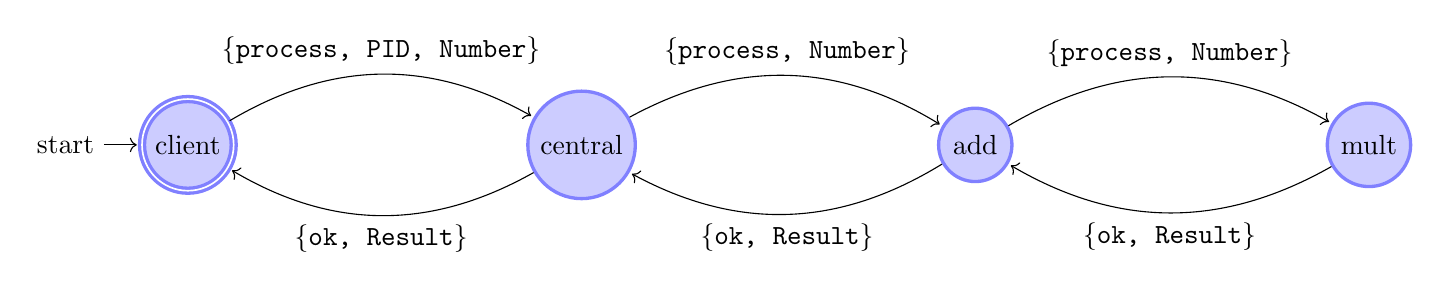
\begin{tikzpicture}[shorten >=1pt,node distance=5cm,on grid,
    every state/.style={draw=blue!50,very thick,fill=blue!20}]
  \tikzstyle{nodeB}=[circle,thick,draw=gray!75,fill=blue!20,minimum size=15mm]
  % States
  \node[nodeB, state, accepting, initial] (q1) {client};
  \node[nodeB, state] (q2) [right=of q1] {central};
  \node[nodeB, state] (q3) [right=of q2] {add};
  \node[nodeB, state] (q4) [right=of q3] {mult};

 
  \path[->] (q1) edge [bend left]  node[above] {\{\texttt{process, PID, Number}\}} (q2);
  \path[->] (q2) edge [bend left]  node[below] {\{\texttt{ok, Result}\}} (q1)
                 edge [bend left]  node[above] {\{\texttt{process, Number}\}} (q3);
  \path[->] (q3) edge [bend left]  node[below] {\{\texttt{ok, Result}\}} (q2);
  \path[->] (q3) edge [bend left]  node[above] {\{\texttt{process, Number}\}} (q4);
  \path[->] (q4) edge [bend left]  node[below] {\{\texttt{ok, Result}\}} (q3);
         
\end{tikzpicture}
}
\caption{Addition and multiplication system}
\label{fig:procadd}
\end{figure}

An interaction with this system can be observed by the following trace:
\[
\begin{align*}
  \sigma \;&=\; \{\text{\texttt{process, <0.1.0>, 10}}\} \{\text{\texttt{process, 10}}\} \ \{ \text{\texttt{process, 20}}\} \ \{ \text{\texttt{ok, 40}}\} \ \{ \text{\texttt{ok, 40}}\} \ \{ \text{\texttt{ok, 40}}\}
\end{align*}
\]

This systems is structured as a pipeline, which is one of the classic
architectures in some \texttt{Erlang} systems, where a process makes a requests
and multiple processes work together in an established order to perform
something over that request. The result will then piggyback to the client after
all the interactions completed. Note that, even if the client has to wait
before performing another request, the system itself is able to deal
asynchronously with multiple clients by spawning processes to deal with each
client request, responding when such process finishes its job.


After augmenting the system with our code injection, the communication flow
changes significantly. Instead of processes interacting directly, all messages
are now routed through the \texttt{conductor}. Every occurrence of
\texttt{gen\_server:call} is transformed into \texttt{conductor:call},
effectively re-directing communication through this intermediary. The
\texttt{conductor} does not alter the contents of the messages; it simply
forwards them to their intended recipients. At the same time, it reports every
observed interaction to a dedicated monitor. This monitor is deployed alongside
the system and receives the messages with their associated context, enabling
runtime property verification. The resulting architecture of the instrumented
system is illustrated in \Cref{fig:procadd-chaos}.

\begin{figure}[ht]
\centering
\usetikzlibrary{arrows.meta, positioning, automata, shapes.geometric}
\scalebox{0.8}{%
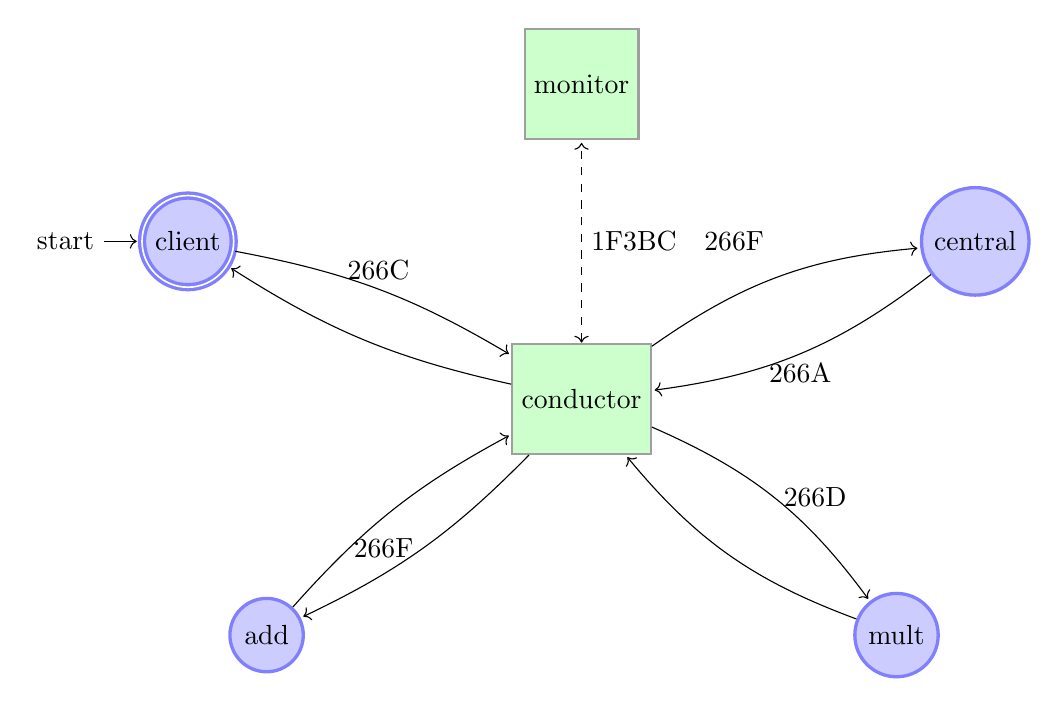
\begin{tikzpicture}[shorten >=1pt,on grid,
    every state/.style={draw=blue!50,very thick,fill=blue!20}]
  % Node styles
  \tikzstyle{nodeB}=[circle,thick,draw=gray!75,fill=blue!20,minimum size=14mm]
  \tikzstyle{nodeSquare}=[rectangle,thick,draw=gray!75,fill=green!20,minimum size=14mm]

  % Conductor + Monitor
  \node[nodeSquare] (cond) at (0,0) {conductor};
  \node[nodeSquare] (mon) at (0,4) {monitor}; % moved further away

  % Processes placed chaotically around conductor
  \node[nodeB, state, accepting, initial] (client) at (-5,2) {client};
  \node[nodeB, state] (central) at (5,2) {central};
  \node[nodeB, state] (add) at (-4,-3) {add};
  \node[nodeB, state] (mult) at (4,-3) {mult};

  % Connections
  % Client <-> Conductor
  \path[->] (client) edge[bend left=10] node[above] {\usym{266C}} (cond);
  \path[->] (cond) edge[bend left=10] node[below] {\musQuarter} (client);

  % Conductor <-> Monitor
  \path[<->, dashed] (cond) edge node[right] {\usym{1F3BC} \ \musQuarter \ \usym{266F}} (mon);

  % Conductor <-> Central
  \path[->] (cond) edge[bend left=15] node[above] {\musQuarter} (central);
  \path[->] (central) edge[bend left=15] node[below] {\usym{266A}} (cond);

  % Conductor <-> Add
  \path[->] (cond) edge[bend left=10] node[left] {\usym{266F}} (add);
  \path[->] (add) edge[bend left=10] node[right] {\musQuarter} (cond);

  % Conductor <-> Mult
  \path[->] (cond) edge[bend left=15] node[right] {\usym{266D}} (mult);
  \path[->] (mult) edge[bend left=15] node[left] {\fl \musQuarter} (cond);

\end{tikzpicture}
}
\caption{Conductor as hub routing all messages}
\label{fig:procadd-chaos}
\end{figure}

Depending on the property that we are monitoring for, the monitor can have a
more complex structure, or follow a simpler \texttt{receive} chain structuring.
A natural property is to verify if the system as a whole behaves correctly,
that is, if the number that a client sends is indeed proceed as expected. In
order to do that we could specify the following property in \texttt{WATLZ}:

\begin{erlang}
OMEGA(
  send {client -> central} WITH {process, _, Number} : TOP;
  send {central -> add} WITH {process, Number1} : TOP;
  send {add -> mult} WITH {process, Number2} : Number2 == Number1+10;
  send {mult -> add} WITH {ok, Result} : Result == Number2 * 2
)
\end{erlang}

The monitor generated for this property is straightforward: it consists of a
sequence of \texttt{receive} statements, each responsible for checking the
property at its corresponding step in the chain.

The experiments were conducted first with a single client interacting with the
system and then with multiple concurrent clients. Across both scenarios, the
outcome is consistent: \texttt{ACTORCHESTRA} introduces noticeable overhead.
This result is expected, as every message must be routed through the
\texttt{conductor}, which assigns context, forwards the message to the intended
process, and simultaneously reports it to the monitor. While this makes the
\texttt{conductor} a performance bottleneck, it is a necessary trade-off for
guaranteeing causality tracking and propagation. The results, shown in
\Cref{fig:singleclientgraphic} and \Cref{table:single_client}, confirm the
theoretical expectation: any architecture that centralizes message handling and
couples it with monitoring inevitably incurs additional cost. Systems that
natively embed causality within their design would experience lower overhead,
but in our case, this mechanism is essential to ensure correctness.

\begin{figure}[htbp]
  \centering
  \includegraphics[width=0.9\linewidth]{Chapters/Figures/Benchmarks/single_client_calc.pdf}%
  \caption{Single Client Performance - Baseline vs Instrumented}
  \label{fig:singleclientgraphic}
\end{figure}

\begin{table}[h]
  \centering
  \small
  \setlength{\tabcolsep}{6pt}
  \renewcommand{\arraystretch}{1.2}
  \sisetup{
    round-mode=places,
    round-precision=1,
    table-number-alignment=center,
    table-format=3.1,
  }
  \rowcolors{2}{rowgray}{white}
  \begin{tabular}{
    r
    r 
    r 
    S[table-format=5,table-number-alignment=center]
    S[table-format=5.1]
    S[table-format=3.1]
  }
    \toprule
    {Clients} & {Req/Client} & {Total Req} & {Baseline (ms)} & {Instrumented (ms)} & {Overhead (\%)} \\
    \midrule
    1 & 500   & 500   & 11.91  & 25.89  & 119.0 \\
    1 & 1000  & 1000  & 21.62  & 42.06  & 95.5 \\
    1 & 2000  & 2000  & 36.61  & 69.14  & 89.6 \\
    1 & 5000  & 5000  & 65.28  & 120.46 & 85.3 \\
    1 & 10000 & 10000 & 102.36 & 209.27 & 105.4 \\
    \bottomrule
  \end{tabular}
  \caption{Single-client benchmark results}
  \label{table:single_client}
\end{table}

The calculator system evaluation reveals important characteristics of our
instrumentation overhead. Under single-client conditions, we observe an initial
overhead of 119\% for light loads (500 requests), which decreases to
approximately 105\% as the system handles heavier loads (10,000 requests). This
trend indicates that our instrumentation exhibits favorable scaling properties,
the relative cost of causal tracking and monitoring does not spike
exponentially as the system processes more requests. The performance of our
system with multiple clients can be visualized in
\Cref{fig:multiclientbench} and the detailed data in
\Cref{table:multi_client_colored}. 

\begin{figure}[htbp]
  \centering
  \includegraphics[width=0.9\linewidth]{Chapters/Figures/Benchmarks/multi_client_calc.pdf}%
  \caption{Multiple Clients Performance - Baseline vs Instrumented}
  \label{fig:multiclientbench}
\end{figure}


\definecolor{pastel2}{RGB}{179, 205, 227}   % pastel blue
\definecolor{pastel4}{RGB}{204, 232, 204}   % pastel green
\definecolor{pastel8}{RGB}{222, 203, 228}   % pastel purple
\definecolor{pastel16}{RGB}{255, 213, 153}  % pastel orange

\begin{table}[ht]
  \centering
  \fontsize{10}{10}\selectfont
  %\footnotesize
  \setlength{\tabcolsep}{6pt}
  \renewcommand{\arraystretch}{1.2}
  \sisetup{
    round-mode=places,
    round-precision=1,
    table-number-alignment=center,
    table-format=3.1,
  }
  \begin{tabular}{
    r
    r 
    r 
    S[table-format=5.1]
    S[table-format=5.1]
    S[table-format=3.1]
  }
    \toprule
    {Clients} & {Req/Client} & {Total Req} & {Baseline (ms)} & {Instrumented (ms)} & {Overhead (\%)} \\
    \midrule
    \rowcolor{pastel2} 2  & 500    & 1000   & 24.75  & 35.10  & 42.5 \\
    \rowcolor{pastel2} 2  & 1000   & 2000   & 42.94  & 69.96  & 63.6 \\
    \rowcolor{pastel2} 2  & 5000   & 8000   & 122.08 & 231.88 & 91.5 \\
    \rowcolor{pastel2} 2  & 10000  & 16000  & 202.77 & 420.83 & 108.1 \\
    
    \rowcolor{pastel4} 4  & 500    & 2000   & 34.71  & 63.65  & 84.4 \\
    \rowcolor{pastel4} 4  & 1000   & 4000   & 57.94  & 95.18  & 65.1 \\
    \rowcolor{pastel4} 4  & 5000   & 16000  & 171.68 & 353.28 & 106.5 \\
    \rowcolor{pastel4} 4  & 10000  & 20000  & 318.02 & 675.57 & 113.1 \\
    
    \rowcolor{pastel8} 8  & 500    & 4000   & 47.49  & 80.82  & 71.1 \\
    \rowcolor{pastel8} 8  & 1000   & 6400   & 73.30  & 128.09 & 75.2 \\
    \rowcolor{pastel8} 8  & 5000   & 20000  & 236.57 & 540.53 & 129.7 \\
    \rowcolor{pastel8} 8  & 10000  & 24000  & 454.58 & 1031.92 & 128.5 \\
    
    \rowcolor{pastel16} 16 & 500    & 6400   & 64.30  & 117.23 & 83.6 \\
    \rowcolor{pastel16} 16 & 1000   & 12800  & 105.13 & 208.88 & 99.7 \\
    \rowcolor{pastel16} 16 & 5000   & 24000  & 492.76 & 1138.48 & 131.7 \\
    \rowcolor{pastel16} 16 & 10000  & 48000  & 945.26 & 2166.70 & 129.6 \\
    \bottomrule
  \end{tabular}
  \caption{Multi-client benchmark results for calculator system}
  \label{table:multi_client_colored}
\end{table}

The multi-client results demonstrate how our instrumentation behaves under
concurrent access patterns. Across different client configurations (2, 4, 8,
and 16 clients), the overhead stabilizes in the 65-131\% range, with most
configurations converging around 100-130\% overhead. Notably, the overhead does
not exhibit exponential growth with client count, indicating our coordination
mechanism scales well with concurrency.

The process of assigning causal context to each message introduces
computational overhead that varies significantly based on request patterns. The
data suggests this overhead is not simply proportional to request volume, but
rather depends on the temporal distribution of requests and the resulting
process scheduling behaviour.
Real distributed systems are inherently concurrent, and our framework
demonstrates that instrumentation overhead remains bounded and predictable
under multi-client scenarios, ranging from 42.5\% to 131.7\%. Crucially, the
overhead does not grow exponentially with increased concurrency, suggesting
that the architecture scales in a controlled manner even under realistic,
concurrent workloads.

% Define pastel colors

\section{Chat System}
\label{sec:chat}

In order to study the impact of our framework in a more complex system, we will
also benchmark the performance overhead over a chat room system, similar to the
one provided in \Cref{sec:waltz_monitor_example}.

The idea of this system is that the clients will register into a main server,
and then they will be able to join different chat rooms and send messages to
those chat rooms. The system would be composed of three main components, the
\texttt{chat\_server} that is the entity communicating with the client, the
\texttt{chat\_room} which will correspond to each chat room created by the
\texttt{chat\_server}, and lastly a \texttt{registry\_server} that will
register and manage the clients into the system. As stated, there will always
be the \texttt{client} entity which serves as the entry point to the
communication with the system. What we will study in this evaluation, are two
different version of this chat system.

The first one, called \texttt{no-broadcast} version, will behave differently
from the \texttt{broadcast} version. Simply put, in the \texttt{no-broadcast}
version, whenever a client posts a message it will simply be logged into a
file, and in the \texttt{broadcast} version we will actually broadcast the
message to all the clients in the room in an asynchronous fashion, using the
\texttt{gen\_server:cast} directive. The interaction schema and the monitored
property are the same as those introduced in \Cref{sub_sec:waltz_chatroom},
namely verifying that all registered clients in the system post messages
exclusively in the rooms they have joined.

\iffalse
The chat system represents a more complex evaluation scenario compared to the
calculator example, as it involves real case communication patterns with
multiple concurrent users exchanging messages. This system particularly
stresses our instrumentation framework because each message must be tracked
through the causal chain, from sender to conductor to receiver, while
maintaining the conversational context that defines proper chat system
behaviour.
\fi
\subsection{No Broadcast Version}
\label{subsec:no_broadcast}
Our evaluation across different client configurations reveals that the message
processing overhead maintains remarkable consistency. As the system scales from
5 clients sending 30 messages each to 200 clients sending 10 messages each, the
overhead stabilizes between 127\% and 145\%. This narrow range demonstrates
that our architecture handles the increased coordination complexity
without exponential performance degradation.

\begin{figure}[htbp]
  \centering
  \includegraphics[width=0.9\linewidth]{Chapters/Figures/NewBenchmarks/no_broadcast_message_time.pdf}%
  \caption{No-Broadcast System: Message Processing Time}
  \label{fig:singleclientgraphicchat}
\end{figure}

The configuration with 200 clients shows the highest overhead at 144.9\%, which
is expected as the conductor must coordinate a larger number of concurrent
message streams. However, the fact that this represents only a 17.7\% increase
over the lightest configuration (5 clients at 127.2\% overhead) indicates
excellent scalability characteristics for our causal tracking mechanism. The
results of the chat system benchmarks are visible in
\Cref{fig:singleclientgraphicchat} and \Cref{table:multi_client_colored_new}.

\definecolor{pastel5}{RGB}{198, 224, 180}
\definecolor{pastel10}{RGB}{255, 205, 210}
\definecolor{pastel20}{RGB}{179, 229, 252}
\definecolor{pastel50}{RGB}{255, 224, 178}
\definecolor{pastel100}{RGB}{197, 202, 233}
\definecolor{pastel200}{RGB}{255, 204, 153}

\begin{table}[h]
\centering
\small
\setlength{\tabcolsep}{6pt}
\renewcommand{\arraystretch}{1.2}
\sisetup{
  round-mode=places,
  round-precision=1,
  table-number-alignment=center,
  table-format=7.3,
}
\begin{tabular}{
  r
  r
  r
  S
  S
  S
}
\toprule
{Clients} & {Msg/Client} & {Total Msg} & {Baseline (ms)} & {Instrumented (ms)} & {Overhead (\%)} \\
\midrule
\rowcolor{pastel5}    5   & 30  & 150   & 38.3   & 87.0   & 127.2 \\
\rowcolor{pastel10}   10  & 30  & 300   & 68.690   & 159.518  & 132.230 \\
\rowcolor{pastel20}   20  & 30  & 600   & 129.403  & 303.401  & 134.462 \\
\rowcolor{pastel50}   50  & 20  & 1000  & 224.911  & 534.313  & 137.566 \\
\rowcolor{pastel100} 100  & 10  & 1000  & 259.799  & 602.706  & 131.989 \\
\rowcolor{pastel200} 200  & 10  & 2000  & 428.1  & 1048.4 & 144.9 \\
\bottomrule
\end{tabular}
\caption{No-Broadcast System: Message Processing Time Table}
\label{table:multi_client_colored_new}
\end{table}

The results are slightly higher compared to the addition and multiplication
system, primarily because that system was a “toy example,” whereas the chat
system reflects the complexity of a real-world distributed environment. Unlike
the simpler case, the chat system requires explicit state management, more
intricate message patterns across processes, and persistent storage, all of
which contribute additional overhead.

Each user triggers multiple instrumented operations across the system, such as
connecting, joining a room, sending messages within that room, joining another
room, and eventually disconnecting. These interaction patterns are considerably
more complex, leading to a higher volume of messages sent to the
\texttt{conductor}.

The increased complexity of the monitor itself also contributes to the overall
system overhead. Unlike in simpler settings, the monitor in this scenario can
spawn sub-monitors to check property satisfaction and route messages to the
appropriate instance. Combined with the higher volume of messages being
funneled through the \texttt{conductor} and the intricate structure of the
monitoring framework, these factors compound the cost. In effect, both the
system’s orchestration and the monitoring infrastructure become more demanding,
amplifying the overhead in this already complex environment.

The latency measurements, presented in \Cref{fig:chatlatency} and
\Cref{table:latency_clients}, reveal the most direct impact of our
instrumentation on user experience. Across all test configurations, the
instrumented version consistently exhibits approximately double the latency of
the baseline system. The latency and throughput measures, were calculated with
the time of the messaging phase of the system, in order to ignore potential
noise and focus on the actual work of the system.

\begin{figure}[htbp]
  \centering
  \includegraphics[width=0.9\linewidth]{Chapters/Figures/NewBenchmarks/no_broadcast_latency.pdf}%
  \caption{No-Broadcast System: Average Latency Comparison}
  \label{fig:chatlatency}
\end{figure}

The chat system evaluation provides additional insights into real-world
performance characteristics. Message processing overhead ranges from 127\% to
145\%, while latency consistently doubles compared to the baseline. Latency
measurements show the instrumented version achieving approximately 50\% of
baseline performance, which represents the most significant impact of our
approach.

\definecolor{pastel5}{RGB}{198, 224, 180}
\definecolor{pastel10}{RGB}{255, 205, 210}
\definecolor{pastel20}{RGB}{179, 229, 252}
\definecolor{pastel50}{RGB}{255, 224, 178}
\definecolor{pastel100}{RGB}{197, 202, 233}
\definecolor{pastel200}{RGB}{255, 204, 153}

\begin{table}[h]
\centering
\small
\setlength{\tabcolsep}{6pt}
\renewcommand{\arraystretch}{1.2}
\sisetup{
  round-mode=places,
  round-precision=1,
  table-number-alignment=center,
  table-format=6.1,
}
\begin{tabular}{
  r
  r
  r
  S
  S
  S
}
\toprule
{Clients} & {Msg/Client} & {Total Msg} & {Base Lat (ms)} & {Instr. Lat (ms)} & {$\Delta$ Lat (\%)} \\
\midrule
\rowcolor{pastel5}    5   & 30  & 150   & 1.0   & 2.6   & 61.5 \\
\rowcolor{pastel10}   10  & 30  & 300   & 2.0   & 4.8   & 58.3 \\
\rowcolor{pastel20}   20  & 30  & 600   & 3.9   & 9.2   & 57.6 \\
\rowcolor{pastel50}   50  & 20  & 1000  & 10.1  & 22.6  & 55.3 \\
\rowcolor{pastel100} 100  & 10  & 1000  & 20.4  & 45.0  & 54.6 \\
\rowcolor{pastel200} 200  & 10  & 2000  & 36.6  & 77.8  & 52.9 \\
\bottomrule
\end{tabular}
\caption{No-Broadcast System: Average Latency Table. $\Delta$ Lat (\%) = degradation from baseline.}
\label{table:latency_clients}
\end{table}

The throughput analysis, depicted in \Cref{fig:chatth} and
\Cref{table:throughput_clients_corrected}, provides insight into the overall
system capacity under our instrumentation. The baseline chat system achieves
throughput ranging from approximately 4,800 to 5,300 messages per second across
different client configurations. Under instrumentation, this drops to a
consistent range of 2,000 to 2,500 messages per second.

The throughput limitation stems from the sequential nature of causal context
assignment in the \texttt{conductor}, each message must be processed to
determine its place in the causal chain before it can be forwarded. 

\begin{figure}[htbp]
  \centering
  \includegraphics[width=0.9\linewidth]{Chapters/Figures/NewBenchmarks/no_broadcast_throughput.pdf}%
  \caption{No-Broadcast System: Throughput Comparison}
  \label{fig:chatth}
\end{figure}

Despite this reduction, the instrumented system still maintains substantial
capacity for development-time evaluation. Processing 2,000+ messages per second
provides ample performance for testing complex interaction scenarios, load
testing with realistic user counts, and validating system behaviour under stress
conditions.

\begin{table}[h]
\centering
\small
\setlength{\tabcolsep}{6pt}
\renewcommand{\arraystretch}{1.2}
\sisetup{
  round-mode=places,
  round-precision=1,
  table-number-alignment=center,
  table-format=6.1,
}
\begin{tabular}{
  r
  r
  S
  S
  S
  S
}
\toprule
{Clients} & {Msg/Client} & {Total Msg} & {Base Thpt (msg/s)} & {Instr. Thpt (msg/s)} & {$\Delta$ Thpt (\%)} \\
\midrule
\rowcolor{pastel5}    5   & 30  & 150   & 5193.5   & 2026.2   & 61.0 \\
\rowcolor{pastel10}   10  & 30  & 300   & 5074.3   & 2082.2   & 59.0 \\
\rowcolor{pastel20}   20  & 30  & 600   & 5176.9   & 2162.6   & 58.2 \\
\rowcolor{pastel50}   50  & 20  & 1000  & 4907.6   & 2180.2   & 55.6 \\
\rowcolor{pastel100} 100  & 10  & 1000  & 4792.2   & 2136.9   & 55.4 \\
\rowcolor{pastel200} 200  & 10  & 2000  & 5272.3   & 2460.7   & 53.3 \\
\bottomrule
\end{tabular}
\caption{No-Broadcast System: Throughput Table. $\Delta$ Thpt (\%) = degradation from baseline}
\label{table:throughput_clients_corrected}
\end{table}

\subsection{Broadcast Version}
\label{subsec:broadcast_version}
When benchmarking our system, we depared ourselves with some very interesting
results regarding the broadcast version of the chat system, which was the
initial implementation that we intended for it. We conducted the same
experiments, with the same configurations and deterministic actions for this
version, and the conclusion can be visible in \Cref{fig:broadoverhead} and
\Cref{table:multi_client_colored_new_broadcast}.

\begin{figure}[htbp]
  \centering
  \includegraphics[width=0.9\linewidth]{Chapters/Figures/NewBenchmarks/broadcast_message_time.pdf}%
  \caption{Broadcast System: Message Processing Time}
  \label{fig:broadoverhead}
\end{figure}

\definecolor{pastel5}{RGB}{198, 224, 180}
\definecolor{pastel10}{RGB}{255, 205, 210}
\definecolor{pastel20}{RGB}{179, 229, 252}
\definecolor{pastel50}{RGB}{255, 224, 178}
\definecolor{pastel100}{RGB}{197, 202, 233}
\definecolor{pastel200}{RGB}{255, 204, 153}

\begin{table}[h]
\centering
\small
\setlength{\tabcolsep}{6pt}
\renewcommand{\arraystretch}{1.2}
\sisetup{
  round-mode=places,
  round-precision=1,
  table-number-alignment=center,
  table-format=7.3,
}
\begin{tabular}{
  r
  r
  r
  S
  S
  S
}
\toprule
{Clients} & {Msg/Client} & {Total Msg} & {Baseline (ms)} & {Instrumented (ms)} & {Overhead (\%)} \\
\midrule
\rowcolor{pastel5}    5   & 30  & 150   & 97.546   & 141.466   & 45.024 \\
\rowcolor{pastel10}   10  & 30  & 300   & 285.502  & 348.611   & 22.105 \\
\rowcolor{pastel20}   20  & 30  & 600   & 930.519  & 1112.422  & 19.549 \\
\rowcolor{pastel50}   50  & 20  & 1000  & 3675.863 & 4079.985  & 10.994 \\
\rowcolor{pastel100} 100  & 10  & 1000  & 7524.454 & 8017.500  & 6.553  \\
\rowcolor{pastel200} 200  & 10  & 2000  & 31209.032 & 32467.304 & 4.032  \\
\bottomrule
\end{tabular}
\caption{Broadcast System: Message Processing Time Table}
\label{table:multi_client_colored_new_broadcast}
\end{table}

Examining the data reveals a markedly different outcome compared to the
\texttt{no-broadcast} version: the observed overhead is significantly lower and
decreases as the workload increases. This behaviour can be attributed to the
amortization of the instrumentation cost across a higher volume of system
activity. In this broadcast scenario, each message is sent to all clients in
the chat room, causing the system’s core workload to grow more rapidly than the
instrumentation overhead. As a result, the relative cost of monitoring
diminishes over time, a dynamic that does not occur in the simpler \texttt{no-broadcast}
version, where instrumentation dominates due to the lower overall workload.

\begin{figure}[htbp]
  \centering
  \includegraphics[width=0.9\linewidth]{Chapters/Figures/NewBenchmarks/overhead_amortization_analysis.pdf}%
  \caption{Instrumentation Overhead: Amortization Analysis}
  \label{fig:amortizedimpact}
\end{figure}

Here, the additional work associated with broadcasting messages effectively
spreads out the monitoring cost of \texttt{ACTORCHESTRA}, demonstrating that in
real-world concurrent systems, the impact of instrumentation can be mitigated.
This efficiency gain is further facilitated by the fact that broadcasts are
handled via the \texttt{cast} OTP directive, a "fire-and-forget" operation that
bypasses the \texttt{conductor}, avoiding extra routing overhead. The effect of
this design choice is illustrated in \Cref{fig:amortizedimpact}.

\iffalse
Examining the data, we observe a clear contrast with the no-broadcast version:
the overhead is significantly lower and even decreases as workload increases.
This phenomenon occurs because the cost of instrumentation becomes amortized by
the system’s real work. In the broadcast version, each message must be
delivered to all clients in the chat room, causing the system’s workload to
grow much faster than the instrumentation cost. As a result, the relative
impact of \texttt{ACTORCHESTRA} diminishes. This effect is further reinforced
by the fact that broadcasts rely on the \texttt{cast} OTP directive, a
fire-and-forget operation not routed through the \texttt{conductor}. The impact
of this amortization is clearly illustrated in \Cref{fig:amortizedimpact}.
\fi



This is also observable in the throughput analysis, as in this broadcast
version the system suffers in the throughput, since the work per message
escalates with the client count, making the system saturated with the broadcast
work, as visible in \Cref{fig:broadth} and
\Cref{table:throughput_clients_broadcast}. Throughput collapses because each
message triggers massive coordination, compared to is counter part, the no
broadcast version, where the system can leverage from concurrency better at
scale due to the non-existent coordination overhead between clients.

\begin{figure}[htbp]
  \centering
  \includegraphics[width=0.9\linewidth]{Chapters/Figures/NewBenchmarks/broadcast_throughput.pdf}%
  \caption{Broadcast System: Throughput Comparison}
  \label{fig:broadth}
\end{figure}

\begin{table}[h]
\centering
\small
\setlength{\tabcolsep}{6pt}
\renewcommand{\arraystretch}{1.2}
\sisetup{
  round-mode=places,
  round-precision=1,
  table-number-alignment=center,
  table-format=7.1,
}
\begin{tabular}{
  r
  r
  S
  S
  S
  S
}
\toprule
{Clients} & {Msg/Client} & {Total Msg} & {Base Thpt (msg/s)} & {Instr. Thpt (msg/s)} & {$\Delta$ Thpt (\%)} \\
\midrule
\rowcolor{pastel5}    5   & 30  & 150   & 1711.1   & 1156.5   & 32.4 \\
\rowcolor{pastel10}   10  & 30  & 300   & 1116.7   & 913.4    & 18.2 \\
\rowcolor{pastel20}   20  & 30  & 600   & 670.0    & 566.6    & 15.5 \\
\rowcolor{pastel50}   50  & 20  & 1000  & 287.7    & 262.4    & 8.8  \\
\rowcolor{pastel100} 100  & 10  & 1000  & 149.1    & 140.8    & 5.6  \\
\rowcolor{pastel200} 200  & 10  & 2000  & 71.4     & 68.7     & 3.7  \\
\bottomrule
\end{tabular}
\caption{Broadcast System: Throughput Table. $\Delta$ Thpt (\%) = degradation from baseline}
\label{table:throughput_clients_broadcast}
\end{table}

These results reveal an important insight: as the workload grows, the cost of
broadcasting messages dominates system performance, gradually overshadowing the
overhead introduced by instrumentation. In practice, this means both versions
of the system converge in runtime behaviour, since broadcasting is the primary
bottleneck. This also accounts for the observed throughput trends, where
scaling introduces a natural degradation effect as message dissemination
becomes increasingly expensive.

\section{Conclusions}
\label{sec:eval_conclusions}

These performance characteristics must be contextualized within the intended
use case of our instrumentation framework. The primary value proposition lies
not in production deployment, but in development-time verification where
runtime property checking provides immediate feedback on system correctness.


During development, engineers routinely tolerate substantial performance
penalties from debugging tools, profilers, and testing frameworks in exchange
for deeper insight into system behaviour. In this context, our measured
overhead of 100–150\% is far from prohibitive, particularly given the unique
advantage it offers: the ability to detect causal property violations at
runtime. Without such monitoring, these issues might remain hidden until late
in deployment or emerge as subtle, hard-to-diagnose bugs in production.

The introduction of an intermediary routing entity fundamentally changes
\texttt{Erlang}'s native message passing semantics. Instead of direct process-to-process
communication, all messages must traverse the instrumentation layer,
introducing additional copying and routing decisions.
Although runtime property verification introduces some instrumentation
overhead, the benefits far outweigh the costs. It enables early detection by
catching issues during development rather than letting them surface as
production failures. It also provides rich causal context, recording the full
sequence of events that led to a violation so developers can understand not
just what went wrong but why. Verification happens automatically, eliminating
the need to manually construct exhaustive test cases for every execution path.
As a result, developers gain greater confidence that their distributed systems
preserve the desired properties, even in complex and highly concurrent
scenarios.

More importantly, in the broadcast version of the chat system the overhead
decreases drastically, ranging from 45\%-4\%, due to the amortized cost of the
underlying operations that a system performs. The conclusion we can take from
this is the overhead impact of our instrumentation depends not only on the
workload applied to the system, but also the whole system architecture itself,
where in some systems the instrumentation cost is what makes a bigger impact
into the system performance, where in others it gets amortized by the true work
load of the system. This makes our framework suitable in real world distributed
systems, where we can mask the potential degradation that the instrumentation
implies.

The same instrumentation framework exhibits dramatically different overhead
profiles when applies to architectures with different computational
complexities per operation. This demonstrates that architecture-workload
interaction is a critical factor in the differences we have seen in the time
executions, where lightweight systems show poor instrumentation amortization,
yet still acceptable for the development and debugging phase, while in more
complex distributed systems, with asynchronous background work, it shows a
better amortization.

\texttt{ACTORCHESTRA} is not a framework to be compared to profiling tools that
do not impact the system in such a way. It is a framework that is used in the
production and debugging phases of development where speed and latency are not
as important as in production. The tool provides complete causality tracking
between messages, and property verification at runtime, catching violations of
properties that other traditional methods might miss. It opens the door to
formal verification in distributed system resolving around the actor-based
model.

Our results also reveal clear avenues for optimization to reduce overhead. The
throughput limitations observed in the chat system indicate bottlenecks within
the monitoring pipeline, which could be alleviated through approaches such as
decentralized conductors or distributed worker pools. Furthermore, the
relatively stable overhead across varying client counts demonstrates the
framework’s inherent architectural scalability, highlighting significant
potential for further refinement and performance improvements.


Rather than serving as a general-purpose commercial monitoring solution, our
framework is intended to complement manual testing and post-hoc debugging. In
distributed systems, where diagnosing subtle bugs can consume days of
investigation, the additional overhead incurred during controlled verification
phases is a worthwhile trade-off. The key consideration is not the overhead
itself, but the value of detecting causality violations early in development.
For many systems, this benefit is substantial. In summary, the framework should
be viewed as a specialized runtime verification tool, tailored for development
and testing scenarios, providing guarantees and insights that conventional
debugging and production monitoring alone cannot deliver.

\iffalse
In this chapter, we will put WALTZ and ACTORCHESTRA to the test. Should we even
compare here the expressiveness with other specification languages in here? Or
simply study the overhead of the tool into our running system. We will explore
two different systems, the one introduced in the begin of the document, a chat
room system, with multiple clients that are processed async by the system (find
another interesting example to explore).

This thesis Monitoring Erlang/OTP Applications using Multiparty Session Types
attacks what we also attack, but follows the multi party paper published by
Nobuko. Worth a read maybe? He follows multi-party sessions types, and tackles
exactly what we tackle, the OTP framework. It has to be compared to our tool, I
think the big difference in our case, is that we start from an original file,
augment it with code injection, and build a new system with causality involved
into it. This work seems to built a system that is already around the sessions
types and the logic is embedded into the implementation. The authors use a DNS
server and a chat system, which is exactly what we could do. This was the
original thesis that I looked at.
\fi

\iffalse
\section{WALTZ vs detectEr}
\label{sec:eval_detecter}
Show the property definition in detectEr and then in WALTZ and how we allow for more expressive monitoring of properties
compared to it. The problem is that detectEr cannot be our only comparison, we need to compare this with other tools, which
I do not know how, because they differ from what we tackle. But, comparing to LTL we might state that it is not possible
to avoid the global state. CTL* is something that Ravara mentioned, might be worth looking into it.
\fi


